\documentclass[a4paper]{article}

\usepackage[english]{babel}
\usepackage{amsmath}
\usepackage{float}
\usepackage{amssymb}
\usepackage{dsfont}
\usepackage{graphicx}
\usepackage{listings}
\usepackage[hyphens]{url}
\usepackage{titling}
\usepackage{varwidth}
\usepackage{hyperref}
\usepackage{color} %red, green, blue, yellow, cyan, magenta, black, white
\definecolor{mygreen}{RGB}{28,172,0} % color values Red, Green, Blue
\definecolor{mylilas}{RGB}{170,55,241}



\usepackage{geometry}
 \geometry{
 a4paper,
 total={165mm,257mm},
 left=20mm,
 top=20mm,
 }

\title{Natural Computing\\Assignment 3}
\author{
  Christoph Schmidl\\ s4226887\\      \texttt{c.schmidl@student.ru.nl}
  \and
  Koen Vijverberg\\ s4132858\\     \texttt{koen.vijverberg@student.ru.nl}
  \and
  Alex Kolmus\\	s4125304\\	\texttt{alex.kolmus@student.ru.nl}
}
\date{\today}

\begin{document}
\maketitle


\subsection*{Swarm Intelligence}

\begin{enumerate}

	% Task 1	
	\item Consider an illustrative example of a PSO system composed of three particles. Consider the following update rule for each particle $i$ and dimension $d$:
	
	\begin{equation}
		v(i;d) = wv(i;d) + r_1(x^*(i;d) - x(i;d)) + r_2(x^*(d) - x(i;d)) \notag
	\end{equation}

To facilitate calculation, we will ignore the fact that $r_1$ and $r_2$ are random numbers and fix them to 0.5 for this exercise. The space of solutions is the two dimensional real values space and the current state of the swarm is as follows

\begin{itemize}
	\item Position of particles: $x_1 = (5,5); x_2 = (8,3); x_3 = (6,7)$
	\item Individual best positions: $x^*_1 = (5,5); x^*_2 = (7,3); x^*_3 = (5,6)$
	\item Social best position: $x^* = (5,5)$
	\item Velocities: $v_1 = (2,2); v_2 = (3,3); v_3 = (4,4)$
\end{itemize}

\begin{enumerate}
	% 1a)
	\item What would be the next position of each particle after one iteration of the PSO algorithm with $w = 2$?\\
	\textbf{Solution:}\\
	
	% 1b)
	\item And using $w = 0.1$?\\
	\textbf{Solution:}\\
	
	% 1c)
	\item Explain what is the effect of the parameter $w$.\\
	\textbf{Solution:}\\
	
	% 1d)
	\item Give an advantage and a disadvantage of a high value of $w$.\\
	\textbf{Solution:}\\
	
\end{enumerate}

	% Task 2
	\item Consider a particle swarm consisting of a single member. How would it perform in a trivial task such as the minimization of $f(x) = x^2$ when $w < 1$?\\
	\textbf{Solution:}\\
	
	
	% Task 3
	\item The figure shows an example from the ACO book by Dorigo and Stuetzle. What results do you expect for ant colony algorithm that does not use tabu lists (except for inhibition of immediate return to the previous node)?
	
		\begin{figure}[H]
	    \centering
  	    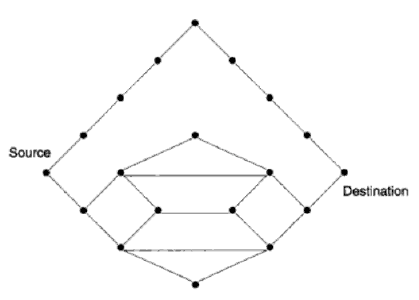
\includegraphics[width=0.4\textwidth]{images/task3.PNG}
	    \end{figure}	
	
	
	\textbf{Solution:}\\
	
	
	% Task 4
	\item Assume that ants are allowed to lay pheromone on a path at every time step, so that pheromone update rule is applied at each time step. Come up with a combination local/global updating scheme that encourages exploration and exploitation - consider which parameters influence this.\\
	\textbf{Solution:}\\
	



	% Task 5
	\item The goal of this exercise is to practice with an implementation of ACO, so please do not use other (possible better) methods for solving this problem.
	
	\begin{enumerate}
		% 5a)
		\item Code an ACO to solve Sudoku's. First, you need to think how to represent Sudoku: there are three conditions an optimal solution must fulfill, each line must contain all integers $\{1,2,3,4,5,6,7,8,9 \}$ once and only once, the same applies to columns and 3x3 subgrids. You can fix one of them so that you will prevent violations. The ACO will have 9x9x9 pheromone matrix, where you update pheromones for the values appearing in the best solutions inversely proportionally to the fitness value. You have to consider also how the old pheromones will fade.\\
		\textbf{Solution:}\\
		
		
		% 5b)
		\item Consider the benchmark Sudoku problems are available at \url{http://lipas.uwasa.fi/~timan/sudoku/}. Run your ACO on the following benchmark instances \textsf{10a.txt, s10b.txt, s11a.txt, s11b.txt}. Report and discuss the results.\\
		 \textbf{Solution:}\\
		
		
		
	\end{enumerate}
	
\end{enumerate}




\end{document}